\documentclass{article}
\usepackage[preprint,nonatbib]{neurips_2021}
\usepackage{graphicx,booktabs,hyperref,array,float}
\makeatletter\renewcommand{\@noticestring}{MH6805 Machine Learning in Finance Group 12}\makeatother
\title{Machine Learning Based Multifactor Stock Selection}
\author{Wu Yangjie \And Zhao Jingjie \And Wang Zhaobo}
\begin{document}
\maketitle
\section*{Research question and real financial data}
Abstract. We compare Logistic Regression, Random Forest, XGBoost and LightGBM for cross-sectional CSI 500 stock selection. We rebuild signals from cached Tushare observations, preserve historical membership and use announcement-based accounting availability. A chronological experiment separates training, validation, testing and later portfolio evaluation. Nonlinear models improve held-out discrimination over the linear baseline, but prediction and portfolio rankings differ. The findings remain conditional on data-vintage and execution assumptions, rather than proving a tradable arbitrage.

1 Introduction. Our question is whether nonlinear interactions between firm characteristics and market signals improve stock ranking over an interpretable linear classifier, and whether statistical gains survive portfolio turnover and transaction costs. We test three hypotheses: fundamentals and market signals provide complementary information; tree ensembles capture useful nonlinearities; and stronger prediction does not necessarily imply higher net investment returns. The project extends earlier internship exploration with a newly rebuilt evaluation pipeline, not a reuse of another module submission.

2 Dataset. Tushare Pro provides daily OHLC/volume, daily\_basic valuation and turnover, adjustment factors, financial indicators, balance sheets, the trading calendar and historical CSI 500 weights. The configured raw window is 4 January 2010 to 30 April 2025. There are 77,034 eligible stock-date rows, 25 factors and 182 usable rebalance dates. Membership is the latest snapshot dated on or before each signal, no more than 62 calendar days old. All raw files have a SHA-256 inventory.

The panel is unbalanced by design. We require a current positive-volume quotation, 60 observed trading records, a valid 60-record momentum factor and no more than 40\% missing features. We do not require a stock to survive to the end of the study. The eligibility filter is determined at signal time, before future returns and labels are known. Financial records older than 550 days become missing rather than being carried indefinitely.

{\small\begin{tabular}{p{.1\linewidth}p{0.18\linewidth}p{0.18\linewidth}p{0.18\linewidth}p{0.18\linewidth}}
\toprule
Split & First signal & Last signal & Dates & Rows \\ \midrule
Train & 2010-05-05 & 2017-09-26 & 91 & 31964 \\
Validation & 2017-10-31 & 2019-03-25 & 18 & 8618 \\
Test & 2019-04-23 & 2020-09-11 & 18 & 8985 \\
Backtest & 2020-10-19 & 2025-04-01 & 55 & 27467 \\
\bottomrule\end{tabular}}
\par\smallskip{\footnotesize Table 1. Chronological samples before purging unavailable training labels.}\par
\clearpage
\section*{Information timing and model selection}
3 Timing and targets. Signals use information available at the rebalance close and trade at the next exchange session open. A filing becomes available no earlier than the calendar day after its announcement; for balance sheets we use the later valid announcement/actual-announcement date. Late amendments to older report periods cannot replace a newer-period filing. Statement end dates never act as release dates. This conservative date lag cannot reconstruct vendor revision vintages, which remain an explicit limitation.

The label is defined from the next execution-open to following execution-open excess return relative to CSI 500. The upper 30\% receive class 1 and the lower 30\% class 0. The middle 40\% are excluded only from binary training and classification evaluation. Every eligible stock, including the middle group and stocks without observable future labels, remains in the scoring/portfolio universe. Scores discriminate the two extreme classes; they are not calibrated probabilities of beating the index.

4 Preprocessing and validation. Each estimator uses the same features and dates. One-percent/ninety-nine-percent winsorization, median imputation and standardization are fitted only on the relevant training fold. No full-panel fallback median is used. Entirely missing training columns become explicit constant-zero transformed columns, not invented source observations. Parameters minimize mean log loss in three expanding chronological training folds, with validation log loss as a tie-break. Any training example whose label exit is not strictly earlier than the next evaluation signal is purged.

Three candidate configurations per model produce 36 training-fold fits, plus validation checks. After freezing parameters, models refit on 23,014 purged training-plus-validation extreme-label rows. Neither test metrics nor later backtest Sharpe selects parameters or factor sets. Ablations reuse the full-factor selected parameters; they are explanatory held-out comparisons, not a second feature-selection exercise.

Logistic Regression tests a linear log-odds specification with L2 regularization. Random Forest averages randomized trees; depth and minimum leaf counts limit variance. XGBoost and LightGBM sequentially fit regularized trees with low learning rates. LightGBM row sampling is explicitly activated using subsample\_freq=1. All random seeds and the finite search grid are saved; the selected settings are not claimed to be globally optimal.

{\small\begin{tabular}{p{.1\linewidth}p{0.36\linewidth}p{0.36\linewidth}}
\toprule
Model & Selected setting & Mean CV log loss \\ \midrule
LR & L2 regularization C=0.01 & 0.7002 \\
RF & 160 trees; depth 4; leaf minimum 100 & 0.6942 \\
XGB & 100 trees; depth 2; learning rate 0.03 & 0.6946 \\
LGBM & 100 trees; depth 2; learning rate 0.03 & 0.6937 \\
\bottomrule\end{tabular}}
\par\smallskip{\footnotesize Table 2. Settings chosen before inspecting held-out results. Full parameter dictionaries are supplied as JSON.}\par
\clearpage
\section*{Held out prediction and ranking evidence}
5 Predictive performance. Table 3 evaluates the same extreme-label test observations for every model. Rank IC is the Spearman correlation between scores and forward excess returns across the full eligible cross-section with observable realized returns. Missing return endpoints are excluded from evaluation, not from the ex-ante investment candidate list. Classification metrics apply to a different, extreme-label population and must be interpreted accordingly.

Random Forest has the strongest test accuracy (54.56\%) and AUC (0.555), compared with Logistic Regression (52.02\%; AUC 0.532). This supports useful nonlinearity, but the gains are modest. Training-only RF accuracy is 57.40\%; the reduction on later observations illustrates the need for temporal validation rather than a claim that overfitting has disappeared.

The ROC curves remain close to the diagonal; discrimination is modest. In the later backtest, RF mean Rank IC is 0.090, with a six-period circular block-bootstrap 95\% interval of approximately [0.046, 0.131]. Blocks use dates, not independent stock rows, to preserve some temporal dependence. This is exploratory evidence from 54 realized holding periods, not a multiple-comparison-adjusted proof of a persistent effect.

{\small\begin{tabular}{p{.1\linewidth}p{0.18\linewidth}p{0.18\linewidth}p{0.18\linewidth}p{0.18\linewidth}}
\toprule
Model & Accuracy & AUC & Log loss & Mean test Rank IC \\ \midrule
LR & 52.02\% & 0.532 & 0.6910 & 0.044 \\
RF & 54.56\% & 0.555 & 0.6878 & 0.081 \\
XGB & 54.23\% & 0.553 & 0.6880 & 0.078 \\
LGBM & 54.00\% & 0.550 & 0.6881 & 0.073 \\
\bottomrule\end{tabular}}
\par\smallskip{\footnotesize Table 3. Independent chronological test metrics. Extreme-label samples only for classification.}\par
\begin{center}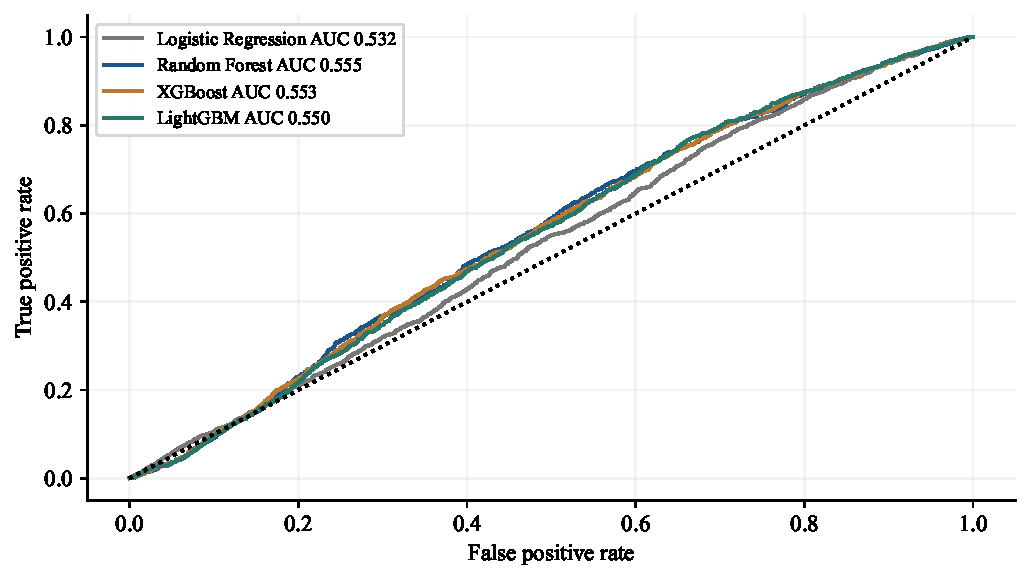
\includegraphics[width=\linewidth,height=3.0in,keepaspectratio]{figures/test_roc.pdf}\end{center}
{\footnotesize Figure 1. Held-out ROC curves use identical observations.}\par
\clearpage
\section*{Daily portfolio outcomes after trading costs}
6 Portfolio construction. The primary portfolio holds the ten highest-ranked stocks at equal target value. A daily ledger uses fractional adjusted-price units, carries locked holdings through suspensions, skips unavailable opening orders without substituting a future-selected stock, and pays 10 bps on absolute buy/sell notional. Weight drift affects actual turnover. Newly available capital stays as cash if an order cannot be executed. Final liquidations incur the same cost where executable; the last period may be shorter than 20 sessions.

Daily values mark suspended positions at their last observed open without altering raw data or model features. Known delisted positions receive a conservative zero recovery at the delisting date. Maximum drawdown includes initial capital 1.0 and uses daily open marks. It is not an intraday worst-loss measure. The benchmark is the CSI 500 price index on exactly the same opening-date interval.

In the later portfolio window, LightGBM records 80.21\% total return and 19.80\% maximum drawdown; RF records 60.04\% and 17.34\%. The benchmark returns -7.32\%. These new outcomes replace the earlier, label-filtered research figures and should not be compared as though only the model parameters changed.

{\small\begin{tabular}{p{.1\linewidth}p{0.18\linewidth}p{0.18\linewidth}p{0.18\linewidth}p{0.18\linewidth}}
\toprule
Model & Total return & Annual return & Sharpe & Max DD \\ \midrule
LR & -1.50\% & -0.35\% & 0.110 & 37.24\% \\
RF & 60.04\% & 11.59\% & 0.683 & 17.34\% \\
XGB & 58.47\% & 11.33\% & 0.674 & 19.20\% \\
LGBM & 80.21\% & 14.72\% & 0.816 & 19.80\% \\
\bottomrule\end{tabular}}
\par\smallskip{\footnotesize Table 4. Long Top 10 net of 10 bps one-way costs. Sharpe assumes zero risk-free return and 252 sessions/year.}\par
\begin{center}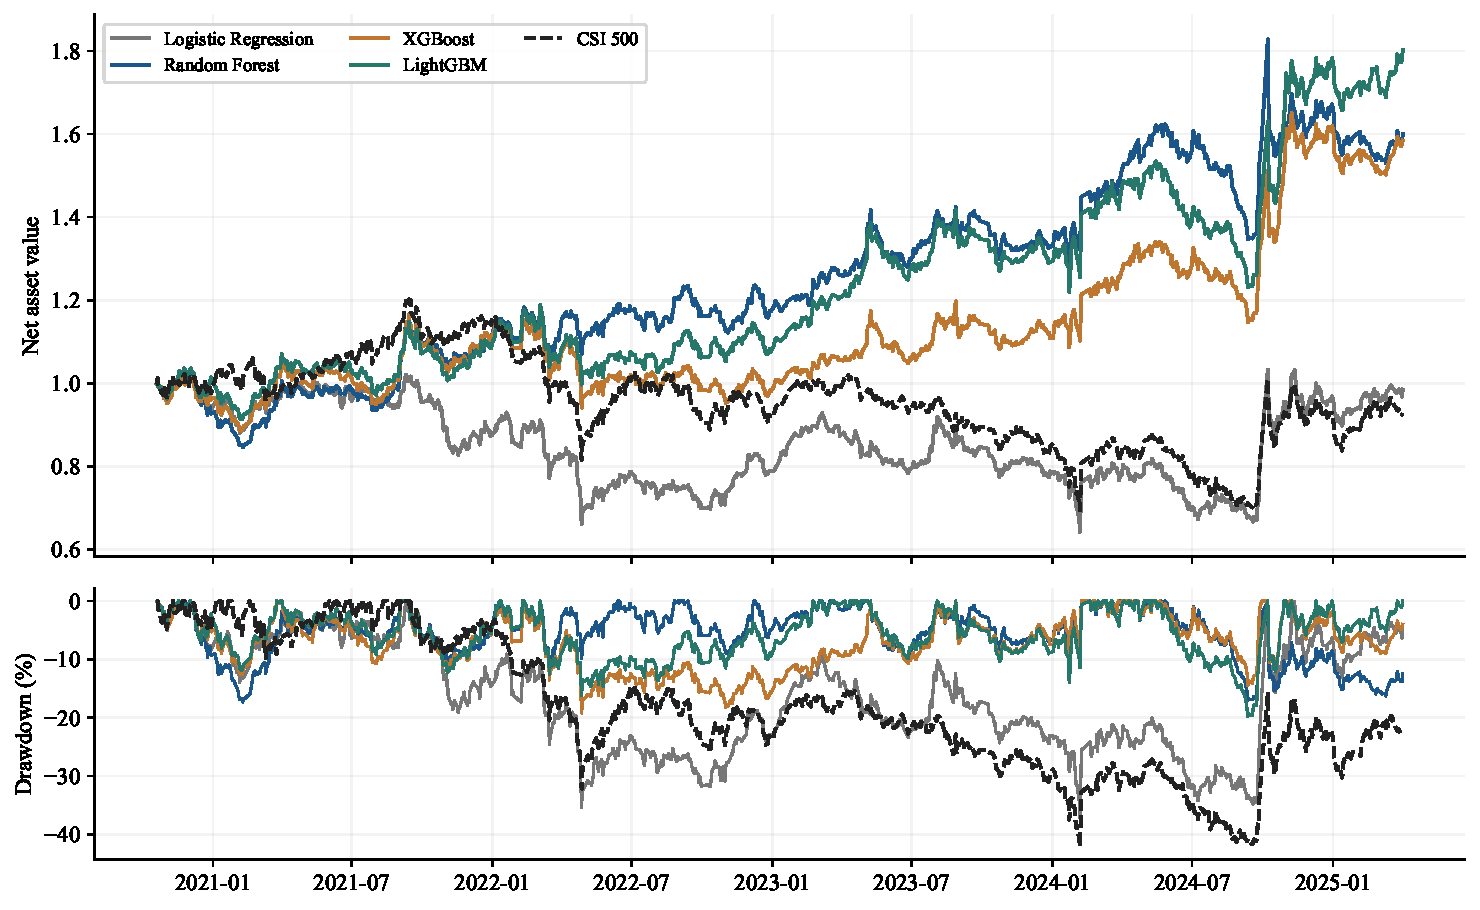
\includegraphics[width=\linewidth,height=3.25in,keepaspectratio]{figures/daily_nav_drawdown.pdf}\end{center}
{\footnotesize Figure 2. Common-period daily NAV and aligned drawdown.}\par
\clearpage
\section*{Factor ablations and model interpretation}
7 Family-level experiments. We refit each model with all factors, fundamentals only, market factors only, and each of seven leave-one-family-out variants. These 40 fits use exactly the same labeled training rows, inference dates and target policy. Hyperparameters remain frozen. The corresponding test-window cost-adjusted portfolio outcomes are also supplied. This isolates information-set effects without selecting the best variant using the test set.

For RF, all factors yield test Rank IC 0.081, versus 0.041 for fundamentals alone and 0.055 for market factors alone. Removing trading/risk factors changes it to 0.042; removing valuation gives 0.099. The combination helps overall, but not every family adds value in this period. An improvement after removing valuation is sample-specific evidence, not a universal rejection of value signals. Correlated factors can substitute for one another.

Permutation importance measures the increase in held-out log loss after independently shuffling one feature. We use a fixed seed, 1,500 real labeled test rows and three repeats for each feature. Importance is predictive, not causal, and can understate correlated substitute variables. We use this explicit importance analysis rather than claiming SHAP explanations that were not computed.

{\small\begin{tabular}{p{.1\linewidth}p{0.72\linewidth}}
\toprule
Model & Three largest permutation importances \\ \midrule
LR & turnover20, roe, grossprofit\_margin \\
RF & turnover20, turnover60, netprofit\_yoy \\
XGB & turnover20, netprofit\_yoy, revenue\_yoy \\
LGBM & turnover20, netprofit\_yoy, netprofit\_margin \\
\bottomrule\end{tabular}}
\par\smallskip{\footnotesize Table 5. Features ranked by increased test log loss; full values and repeat standard deviations are supplied.}\par
\begin{center}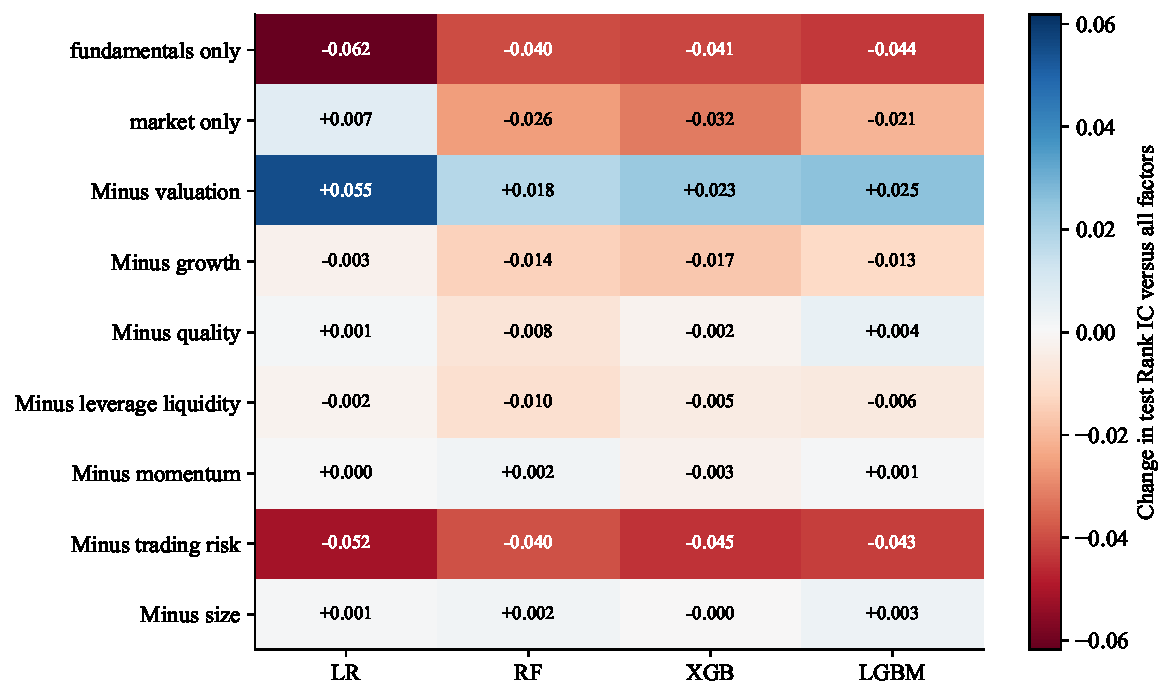
\includegraphics[width=\linewidth,height=3.1in,keepaspectratio]{figures/factor_ablations.pdf}\end{center}
{\footnotesize Figure 3. Test Rank IC change relative to each model with all factors.}\par
\clearpage
\section*{Turnover costs and stability over time}
8 Robustness. All models use the same predeclared one-way costs: 0, 5, 10 and 20 bps, without selecting parameters using these curves. Calendar slices use common opening dates; 2020 and 2025 are partial. LightGBM returns 38.0\% in 2024 and -1.7\% in 2022, while RF returns 5.2\% in 2022. Such differences show why aggregate returns alone cannot establish stability.

Ten score-sorted portfolios include every eligible candidate, and their daily ledgers also deduct transaction costs. Group 1 has the lowest score and group 10 the highest. We examine the direction and smoothness of the decile profile rather than demanding perfect monotonicity or presenting a large long-short loss as the drawdown of every group.

Supplementary hedged portfolios use a clearly normalized 50\% long / 50\% short daily return-spread convention with 100\% gross exposure. One hedge subtracts CSI 500 returns and the other subtracts the bottom-stock sleeve; hedge costs are explicitly charged. These are diagnostic overlays, not executable short-sale or futures strategies. Borrow availability, funding, margin, stock limits and futures basis/roll are not fully represented, so the long-only portfolio remains the primary investable approximation.

\begin{center}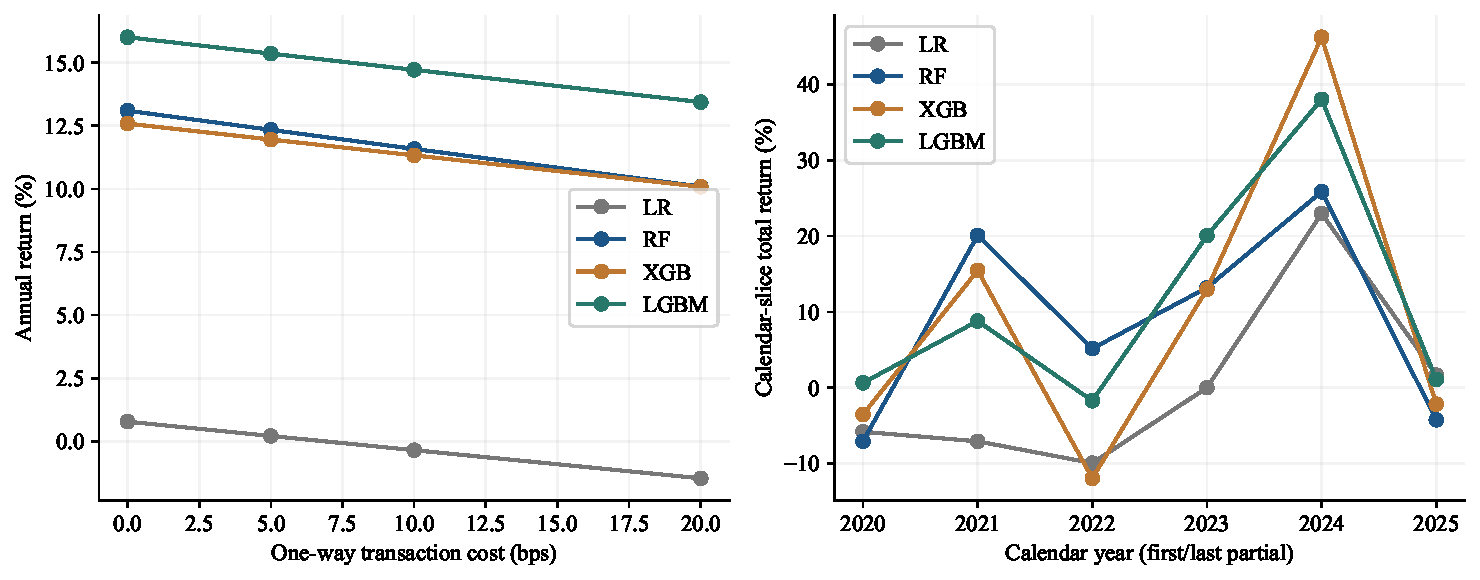
\includegraphics[width=\linewidth,height=2.05in,keepaspectratio]{figures/costs_and_subperiods.pdf}\end{center}
{\footnotesize Figure 4. Cost sensitivity and calendar-slice returns, without tuning on the displayed results.}\par
\begin{center}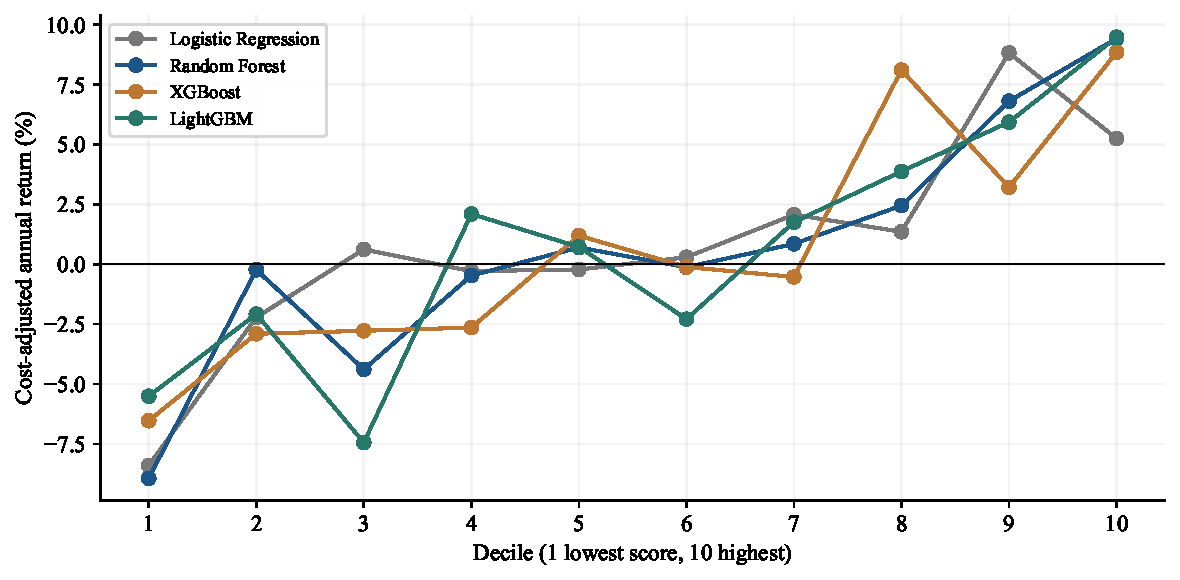
\includegraphics[width=\linewidth,height=1.9in,keepaspectratio]{figures/decile_returns.pdf}\end{center}
{\footnotesize Figure 5. Net annual returns of all ten score groups.}\par
\clearpage
\section*{Discussion limitations and references}
9 Discussion. The test evidence favors tree ensembles over the linear baseline, but the highest classification score does not identify the highest-return Top 10 portfolio. Classification loss averages errors across labeled extremes, whereas a concentrated portfolio depends on the ordering and realized tails of only a few names. Turnover, volatility and regime sensitivity therefore matter alongside AUC. We do not claim that boosting is universally superior to Random Forest.

Information timing controls remove several avoidable sources of leakage: report-period end dates are not release dates; preprocessing uses only training data; training label horizons are purged; and future-return labels never define the inference universe. These corrections materially change the experiment. They do not turn cached vendor data into a certified historical-vintage database.

Limitations. Cached financial statements may contain revisions not identifiable from the retained date fields. Historical constituent snapshots have publication/staleness uncertainty. Early-period financial coverage reduces the eligible universe and is reported rather than hidden. Daily-open execution lacks auction fills, price-limit and lot-size rules, market impact and cash-dividend accounting in actual shares. Suspension marks can temporarily understate risk, zero delisting recovery is conservative, and index price returns differ from a total-return benchmark. The small chronological test sample, finite parameter grid, correlated features and many exploratory comparisons limit statistical certainty.

Future work should validate financial vintages, introduce execution and borrow data, test a frozen walk-forward protocol, and assess capacity and uncertainty before any live deployment. Existing out-of-sample outcomes are research evidence under stated assumptions, not a promise of future returns.

Contribution statement. Wu Yangjie, Zhao Jingjie and Wang Zhaobo contributed equally to this group project.

\section*{References}
{\footnotesize Breiman, L. (2001). Random Forests. Machine Learning 45, 5-32. https://doi.org/10.1023/A:1010933404324\par}
{\footnotesize Chen, T. and Guestrin, C. (2016). XGBoost: A Scalable Tree Boosting System. https://arxiv.org/abs/1603.02754\par}
{\footnotesize Ke, G. et al. (2017). LightGBM: A Highly Efficient Gradient Boosting Decision Tree. NeurIPS 30.\par}
{\footnotesize Tushare Pro API documentation. Daily: https://tushare.pro/document/2?doc\_id=27 ; daily\_basic: https://tushare.pro/document/2?doc\_id=32\par}
{\footnotesize Financial indicators: https://tushare.pro/document/2?doc\_id=79 ; balance sheets: https://tushare.pro/document/2?doc\_id=78\par}
{\footnotesize Trading calendar: https://tushare.pro/document/2?doc\_id=26 ; historical index weights: https://tushare.pro/document/2?doc\_id=96 ; adjustment factors: https://tushare.pro/document/2?doc\_id=28\par}
\end{document}